\chapter{Preliminaries}\label{preliminaries}
This section will describe malware, the different types and how it utilizes DGA perform malicious act. It will also explain the basics of machine learning and different types of neural networks that are necessary for this research paper to know. \\\\  
Malware is a blending of two words, malicious and software, where it clearly defines the functionality of it, namely a software that is malicious in nature. Malware can have multiple purposes. Cybercriminals typically use it to extract data from the victims computer to leverage against them for financial gain. This data can range from financial data, sensitive personal data: such as healthcare records, personal emails, passwords, etc. The possibilities of the information that can be compromised are endless.\\\\ 
The most common ways victims receive malware is through the internet and mail.Malware can penetrate a victim's computer in different ways, such as: surfing to hacked websites, viewing malicious ads on websites, download infected files and install malicious programs or apps. When a malware has infected the computer system of a victim, it can come in many forms, such as Ransomware, Spyware, Trojans, Worms, etc.

\section{Botnets}
A compromised machine that is infected by malware can end up a network of infected machines (botnets). This machine is a bot in that network that receives and responds to commands from the command \& control server. The C \& C server is controlled by and receives commands by a human controller called a botmaster. The botmaster conceals itself by employing
a number of proxy machines, called the stepping stones, between it and the C \& C server. The life cycle of a botnet can be divided into four phases. For this research only the first two phases are important. The first phase is when the machine (bot) receives the malware and executes the binary.
After the machine is infected, this machine (bot) tries to contact the C \& C server to announce its presence and contact with it. This establishment phase is called Rallying. There are two ways that the bot can contact with the C \& C server. The first way that the bot knows the IP address of the C \& C server. This IP address can be hardcoded into the binary, which can be exposed by reverse engineering the binary. The IP address can also be seeded, where the bot is provided by a list of peers, this list can be hidden in Windows registries.  The second way is that the bot knows the domain name of the C \& C server.  The domain name can be hardcoded into the bot binary, where it can resolve to different IP addresses.  Reverse engineering this binary may expose
the domain name, which can then be blacklisted.

\section{Domain Generated Algorithm}
The domain name can also be generated, then the bot dynamically contacts the C \& C server using DGA (Domain name Generation Algorithm). The essence of this algorithm is that it creates a set of random strings. The bot attempts to resolve the generated domain names by sending DNS queries until one of the domains resolves to the C \& C server IP Address. The domains that do not resolve will result in Non-Existent Domain (NXDomain) responses.\\\\ 
The domain names that are generated by the DGA are also known as Algorithmically Generated Domains (AGD). The DGA uses a seed to serve as a shared secret between the botmaster and the bot. There are two types of seeds: static seed and dynamic seed. The seed is required to calculate the AGDs. The DGA takes the seed value as input to generate pseudo-random strings and append algorithmically TLD (Top Level domains) such as \textit{.nl, .com, .org, .edu}. The static seed can be dictionary of words, random strings that are concatenated, numbers or any other value that the botmaster can come up with. Dynamic seeds are dynamic, it changes with time. Dynamic seeds can be currency exchange rate, daily trending twitter hashtag, weather temperature and current date and time.  The static and dynamic seed elements are then stitched together to generate a pseudo-random string.\\\\ 
The botmaster uses the DGA to generate a large number of domain names for the C \& C server.  The constant change of domain names for the C \& C server using DGA is known as Domain-Fluxing.  The botmaster registers one of the DGA created domain names for the C \& C server in advance using the same algorithm of the DGA.  When the bot receives the malware, the malware queries to the pre-registered domain name and resolves the IP address using DNS.  The botmaster registers the domain name most of the time some hours prior to an attack and disposes of the domain names within a day.  Whenever the previous domain name that the bot connected with does not resolve anymore, it queries to the next set of generated domain names until it find one domain that works.\\\\ 
The DGA and constant domain-fluxing of the C \& C server provides agility and resilience to the infrastructure of the botmaster.  This makes it hard to predict what domain names a bot will try. Analyst will re-engineer DGA by analyzing the malware and understand how the algorithm works. It is still hard to predict what kind of seed the DGA will use on a specific time. It is also infeasible to report all the domain names that are generated. As some DGA use english dictionary as static seed values, it is hard to distinguish benign domain names from malicious ones. 

\section{Machine Learning}
Machine learning has recently been an attractive tool to be used in security. One way to combat DGA is to use machine learning to find the structure of the generated domains. The machine learning methods can be either supervised or unsupervised. Unsupervised learning uses algorithms to analyze and cluster data, in this case the domains. These algorithms discover hidden patterns or data groupings, without a need for a human intervention. There are three ways to approach unsupervised learning: clustering, association and dimensionality reduction. The domains are divided into clusters to find statistical attributes for each group. To produce a cluster with good generalization capabilities, it can take a lot of time and  effort \cite{Unsupervised}. Supervised learning does not rely on the statistical attributes  for each group to find DGAs. Supervised learning attempts to understand and classify the input and predict the outcome accurately. The relationship is represented as a structure to predict the outputs for some specific future inputs.

\section{Neural Networks}
Artificial Neural Networks are artificial systems that were inspired by the biological counterpart. The systems learn in a supervised manner to perform tasks by using various datasets and examples. These neural networks are composed of node layers, containing one or more input layers, hidden layers and output layers. Each node is connected to another node and has an associated weight $w$ and threshold $t$. When the threshold of a specific node is above a certain threshold value, then that node is activated, otherwise no data is passed along to the next layer of the network. This is determined by a specificly used activation function in the network. \\\\ 
The network uses training data to learn and improve the accuracy of the network. This is usually done by backpropagation. Backpropagation is a supervised learning algorithm that computes the difference between the model output and the actual output using gradient descent and the chain rule . It checks if the error is minimized and update the weights and biases accordingly. It repeats the process until the error becomes minimum \cite{Gradient_Descent}.


\section{Activation Functions}
The activation functions in a neural network are functions that determine the output of a neural network. It maps it to a specific value. The function receives the calculated weighted sum of the inputs and the added bias and then decides if this passes through or not. \\\\
There are two types of activation functions: Linear Activation function and Non-linear Activation Functions.
The linear activation functions are functions that does not change the weighted sum of the input, but instead returns the value directly. For multiple layer networks we need non-linear activation function.

\subsection{ReLU}
ReLU, or Rectified Linear Unit, is linear when the input is positive and 0 when the input is negative. The range of ReLu is [0, inf). The benefit of ReLu is that there is a reduced likelihood of the gradient to vanish(see subsection Vanish Gradient Problem), as the gradient is constant. This constant gradient results in faster learning of the network. Another benefit is the sparsity, as the network has more units in a layer, other activation functions will be processed to describe the output of that network. When the calculated sum that goes into the activation of ReLu is negative, it yields 0. This means there is fewer neurons firing, which makes the network lighter.\\\\
The disadvantage is that it tends to blow up, as the range goes to infinity and there is no mechanism to constrain the output when it is positive. Another disadvantage is the problem that if too many activations in the network get below zero, than the neurons in the network will output zero. This means that the outputs die out, thus prohibiting learning. This is called the Dying ReLu problem.

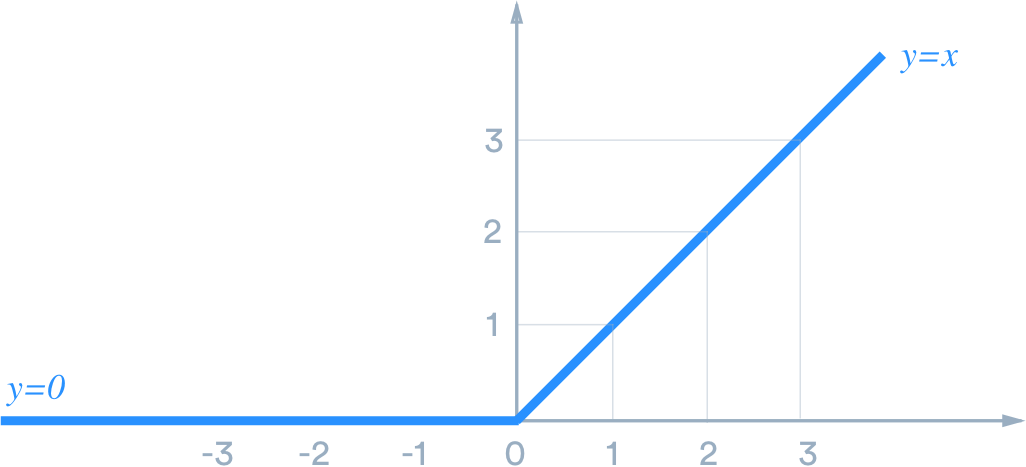
\includegraphics[width=10cm]{relu}

\subsection{Sigmoid}
Sigmoid activation function is a non-linear activation function that looks like an S-shape. Any small changes in the incoming X value(the calculated sum) will cause the Y value (the output) to change significantly. The range is [0,1], so it is bounded in a range and it does not blow up. The disadvantage of the Sigmoid function is the vanishing gradients(see subsection Vanishing Gradient Problem)

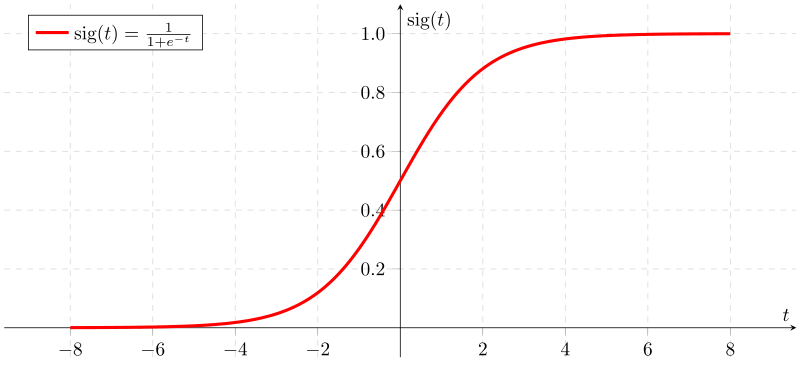
\includegraphics[width=10cm]{sigmoid_function}

\subsection{Tanh}
The Tanh activation function is very similar to the Sigmoid function. The difference is that the range is [-1,1] and the gradient is stronger for tanh than sigmoid. That means the derivative are steeper. One benefit of tanh over sigmoid is that it avoids bias in the gradients \cite{Tan_h}.

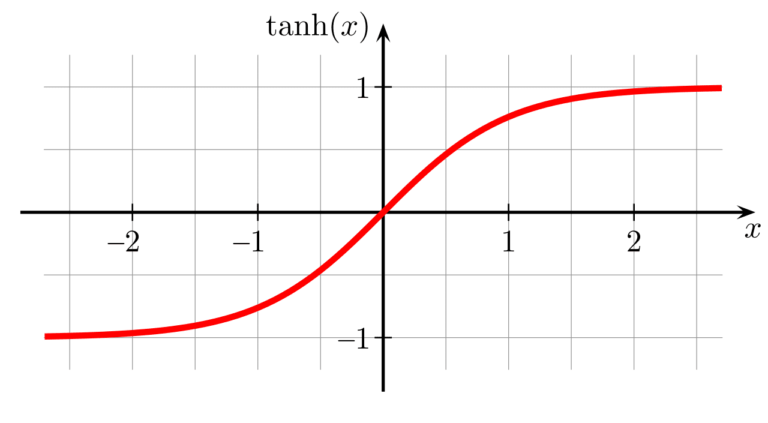
\includegraphics[width=10cm]{tanh_function}

\section{Recurrent Neural Networks}
Recurrent neural networks or RNN, are a type of neural network that uses the output from the previous step and fed that as input in the current step, while in traditional Neural networks the network assumes that the inputs and outputs are independent of each other. The cost function or error can be calculated at any time $t$. At any given time $t$, the current input is a combination of $x_t$ and $x_{t-1}$. This makes the neural network recurrent, it has feedback loops at each iteration of the hidden layer. One thing Recurrent Neural Networks are used for are Sequence Modeling. Sequence Modeling is the task to predict about future outcomes.\\\\
There are some drawbacks to RNN. The first drawback is that when the sequence is looked at in order, there will be a limit in how much parallelize training can be done. The second drawback is that the farther away the relevant points in the sequence are from one another, the harder and slower it is to make connections between them. This drawback is caused by the vanishing gradient problem.\\

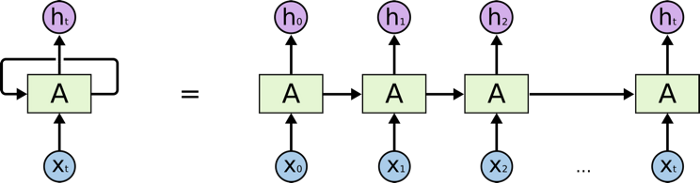
\includegraphics[width=12cm]{RNN}

\subsection{Vanishing Gradient problem}
The vanishing gradient problem can be encountered when gradient-based learning methods and backpropagation is used. As there are more layers using activation function are added to the neural network, the gradients of these loss functions approaches zero. The gradient will be vanishingly small, which in turn prevents the current weight from changing its value. This can lead to the neural network to stop further training. As mentioned before, an activation function like the sigmoid function, squishes a large input space into a value between 0 and 1. The effect of this is that a large change in input would cause a small change in the output. The derivative therefore becomes very small. The derivative approaches zero, which causes the gradient of this layer in the network to vanish.\\\\
As mentioned above, one network that suffers from vanishing gradient problem is a traditional Recurrent Neural Network. When the feedback loops occurs and the gradient is getting lower, then it is more harder for the network to update it weights. The weights of the initial value will not change effectively through the training process, which can lead to inaccuracy in the network. \\\\
The solution to the vanishing gradient problem is to use other activation functions for the network, such as ReLu, which doesn't cause a small derivative. Another solution is to use residual networks \cite{DBLP:journals/corr/HeZRS15}. There are also specialized RNNs, that are resistant to this problem. One of these architectures is the Long short-term memory (LSTM) network. 

\subsection{LSTM}
Long short-term memory (LSTM) is a specialized RNN, that is capable of learning in long-term dependencies. It is designed to remember information for long periods of time. It does that by adding a forget mechanism. The hidden layer in LSTM is a gated cell. It consists of four layers that interact with each other to produce the output of that cell to pass on to the next hidden layer. LSTM is compromised of three logistic sigmoid gates and one tanh layer, compared to traditional RNNs that use only single layer of tanh. These gates are used in order to limit information or pass information through the cell. The inputs of LSTM go through the input gate, forget gate and output gate. The forget gate decides to remember or to skip inputs from the previous hidden states. The mechanism of the forget gate mostly solves the vanishing gradient problem. The input gate decides what new information has to be added to the cell. Finally the output gate decides which new information or old information has to be passed to the next hidden layer by using the memory state that are updated by the input and forget gate.\\

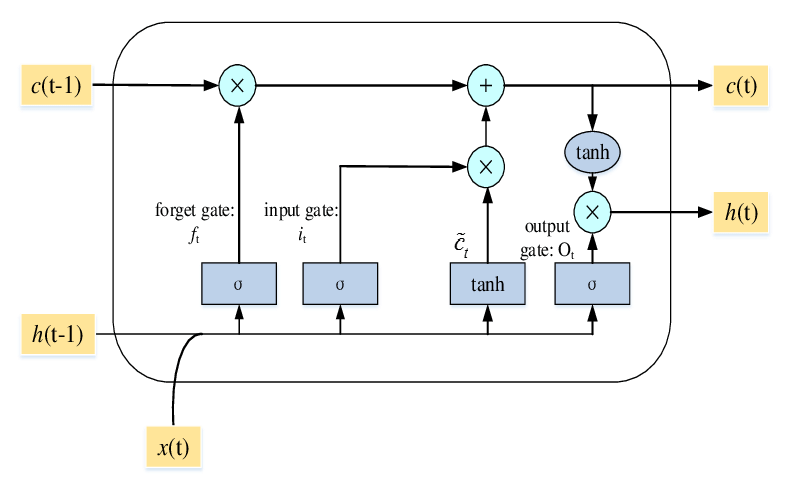
\includegraphics[width=12cm]{LSTM}
\\ While LSTM overcame the vanishing gradients in the network, it still inherits some problems of RNNs, such as: no parallelization, as there is still a sequential path for the data. LSTMs was created to solve the vanishing gradient problem, but it could not remove this problem completely. This is because the data still has to move from cell to cell in a sequential manner. The problem inherently lies in the recursion of RNNs. Also LSTMs are even slower to train than traditional RNNs, as they are more complex than traditional RNNs.

\section{Transformers}
A transformer is a new deep learning model that the input sequence can be passed in parallel, which can increase the speed drastically. In the paper \textit{"Attention is all you need"} \cite{Transformers} the transformer was first introduced. In that paper it explains how transformers using self-attention layers. Attention is a mechanism that finds out how relevant all the other tokens are in a sequence for a given token. Attention learns to weight the relationship of each token in the input sequence to other tokens in the output sequence. Self attention is similar, but it allows inputs to interact with each other as well. In the paper the transformer model uses multi-headed attention layers. In multi-headed attention, each head in the layer learns attention relationship independently. Attention is a combination of three matrices that are combined together, where every value in that matrices are learned.\\\\
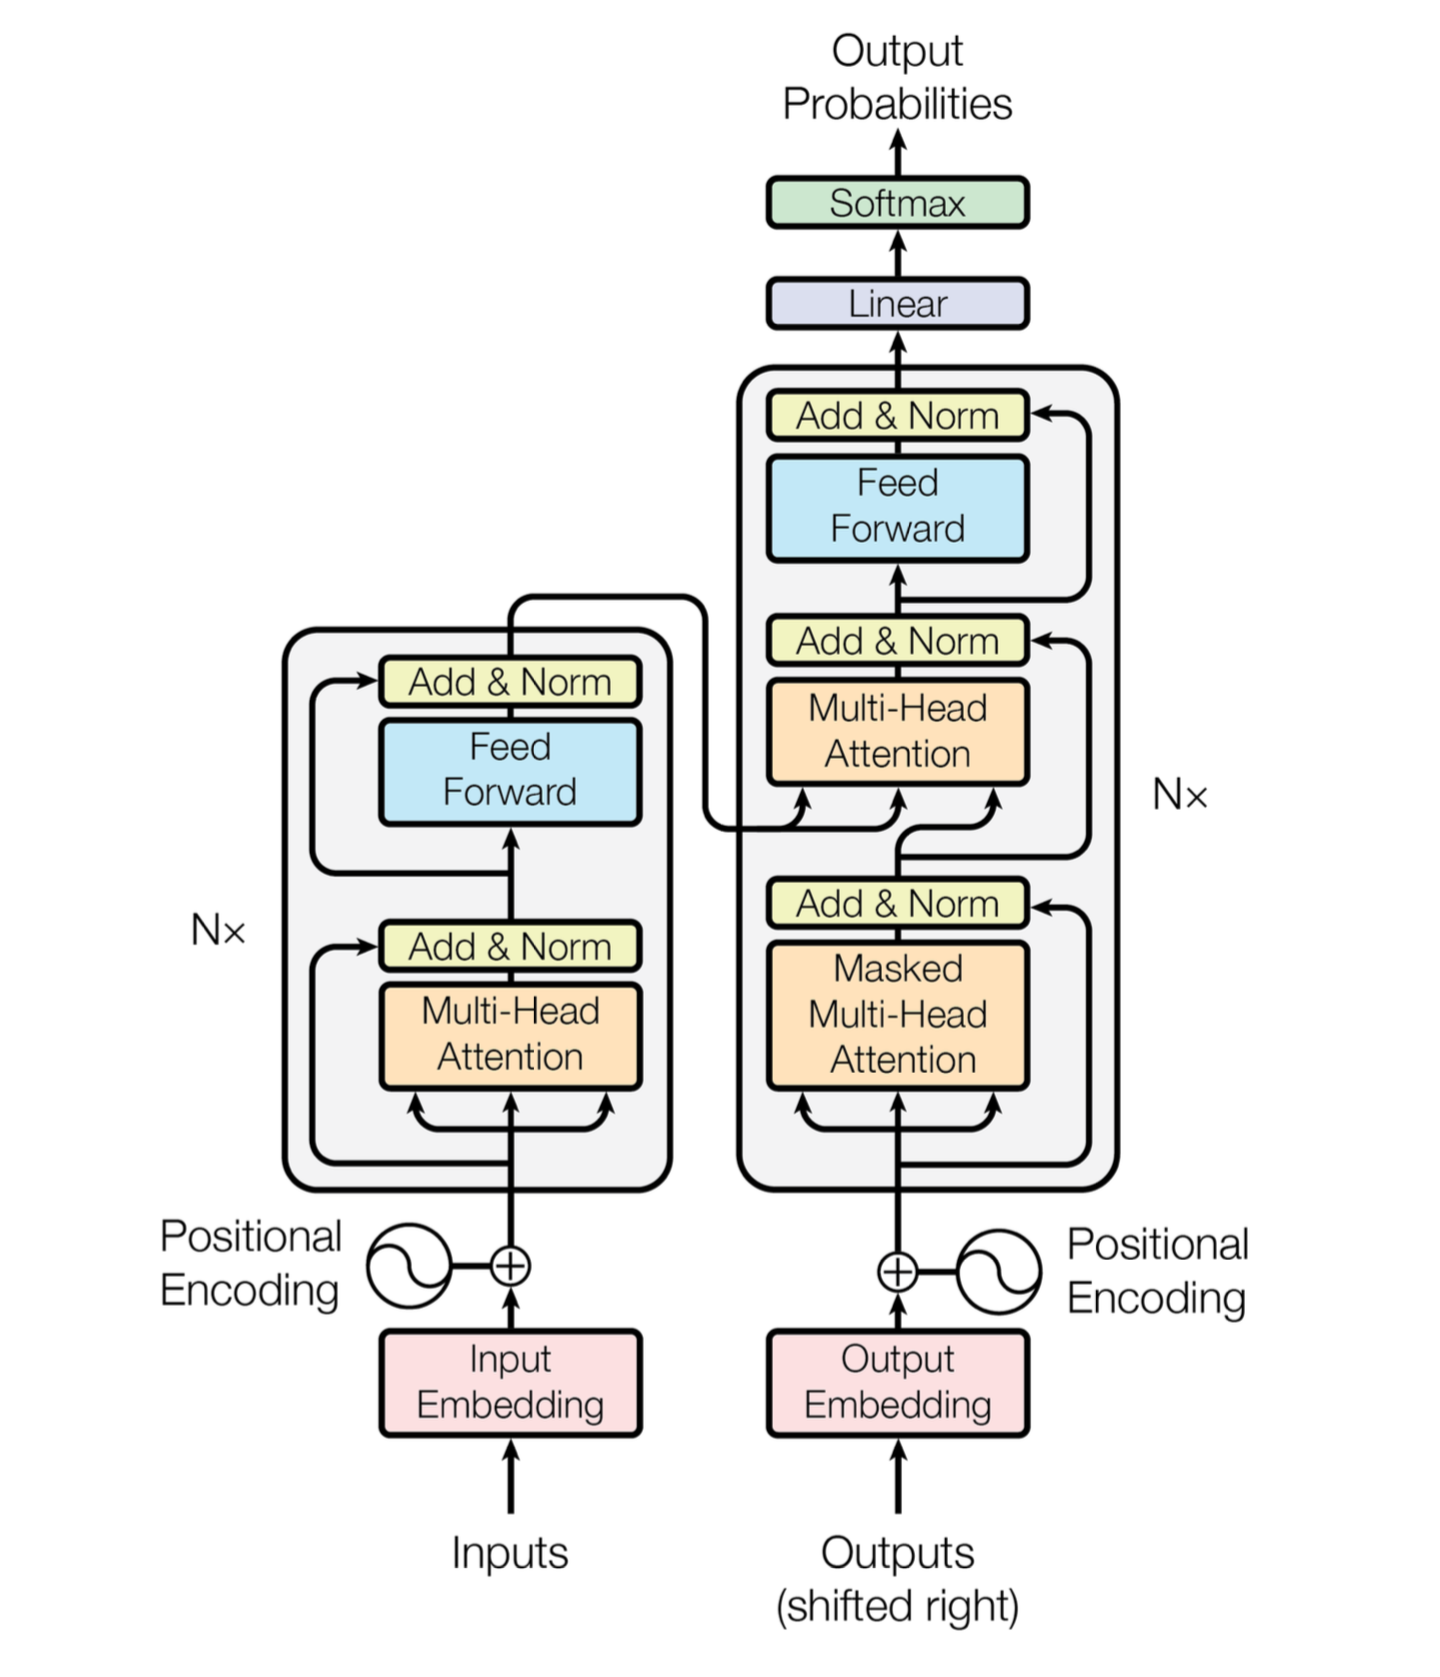
\includegraphics[width=12cm]{transformer}
The transformer architecture that was purposed by the paper, uses a sequence to sequence model \cite{sts} that has an encoder and a decoder. Before the inputs go into the encoder, the input has to be embedded. Input embedding maps every word to a point in space where similar words or meaning are physically closer to each other. This space is called the embedding space. The embedding space maps a word to a vector. In a sentence same words can have different meaning. That is why in a transformer there are positional encoders. This is a vector that gives context based on position of word in sentence. By adding the position encoding we will get embedding of words with context information. This input embedding with context then goes to the Encoder. This encoder contains a stack of multi-headed attention and a feed-forward neural network \cite{ffn}. These feed-forward neural network are used to transform the attention vectors to make it digestible for the next encoder or decoder block. The decoder is similar to the encoder, only it has an additional multi-head attention block. Transformers are used for Sequence to Sequence tasks like NLP or machine translation. It can also be used as embedding using approaches like masked language modelling. One of these models, created by Google, is called BERT.

\subsection{BERT}
BERT (Bidirectional Encoder Representations from Transformers) is a large transformer masked language model. It is mostly used for pre-training natural language processing (NLP). The main innovation of this technique is applying bidirectional training on a Transformer model. In contrast, other efforts looked at it in a single direction, from left to right or right to left. \\\\
BERT only uses the encoder mechanism to generate a language model. The encoder of BERT reads the entire sequence of words at once. That ensures that the model learns the context of a word from all its surroundings, thus making it bidirectional. BERT are pretrained on two tasks: language modelling (LM) and next sequence prediction (NSP). It uses Masked LM (MLM) for pretraining language modelling. This is done by replacing 15\% of any sequence with a [MASK] token. The model tries to predict the original value of the masked words, using the context provided by the other non-masked words in a sequence. Masked language models are a kind of contextual word embedding models. Contextual word embedding gives a model different representation for different sentences.\\\\ 
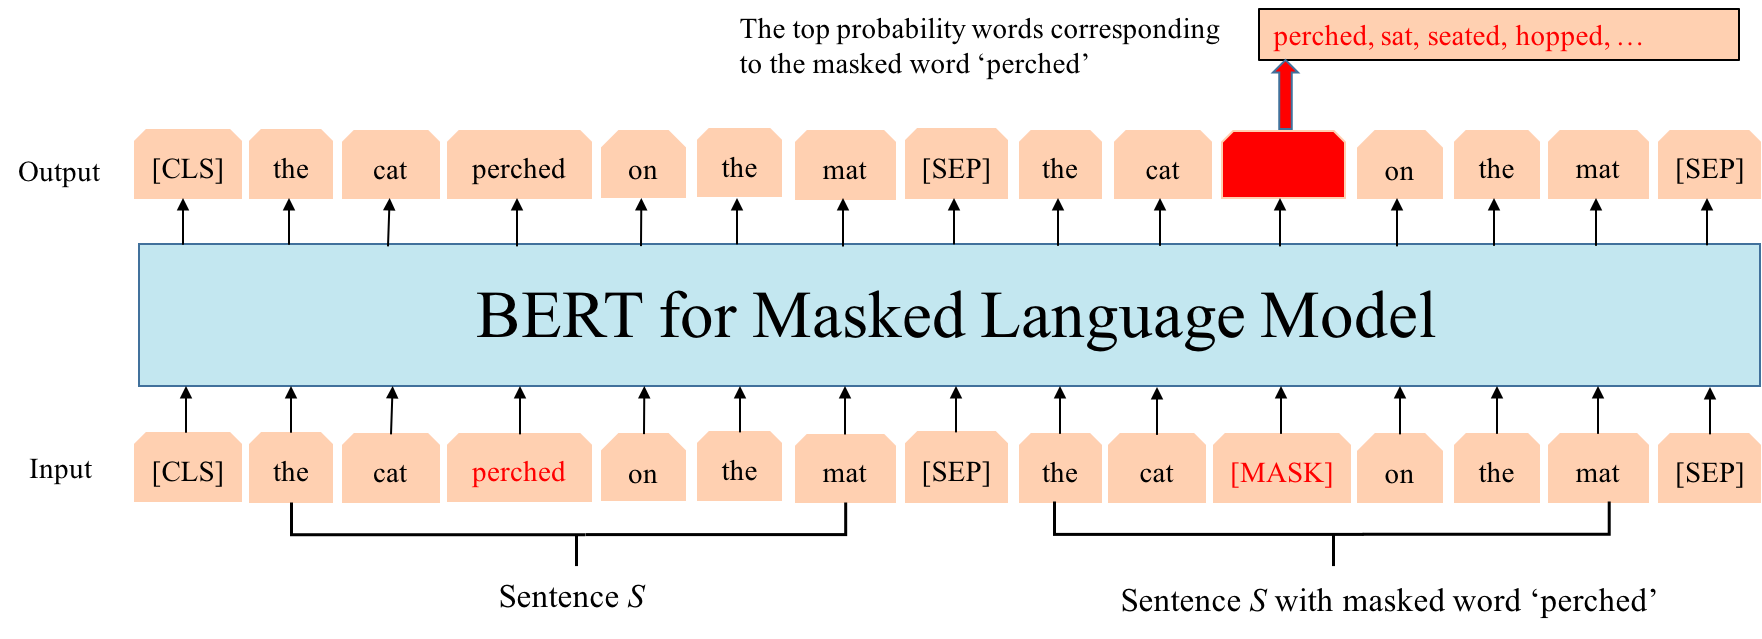
\includegraphics[width=10cm]{BERT}
\\\\ The next task of the training process, BERT uses next sentence prediction to understand the relationship between two sentences. The model receives as input pairs sentences and it learns to predict if the second sentence is the next sentence in the original document. BERT separates sentences with a special [SEP] token. Then the model is fed with two input sentences at a time. During training, 50\% of the time the second sentence is the subsequent sentence in the original document, while in the other 50\% of the time it is a random sentence from the full corpus. The assumption being that the random sentence will be disconnected from the first sentence.
All together the input in BERT is processed in these steps:
\begin{enumerate}
    \item Each sentence sequence is separated by a [SEP] token. It is placed at the end of each sentence.
    \item Every sentence will replace 15\% of its words with a [MASK] token.
    \item At the beginning of the first sentence a special [CLS] token will be inserted.
    \item Every other word in a sentence is transformed into an embedded token.
    \item A sentence embedding is added to each token. They are similar in concept as token embeddings, but these embeddings are used to indicate if sentence A or sentence B is added to each token.
    \item At last a positional embedding gets added to every token to indicate their position in the sequence.
\end{enumerate}
